\documentclass{beamer}
\usepackage[utf8]{inputenc}
\usepackage[spanish]{babel}
\usepackage{amsmath}
\usepackage{graphicx}

\usetheme{Madrid}
\usecolortheme{whale}

\title[Regresión Logística]{Módulo 4: Aprendizaje Automático}
\subtitle{Clase 4: Regresión Logística y Clasificación Binaria}
\author{Diplomado en Ciencia de Datos}
\date{\today}

\begin{document}

\begin{frame}
    \titlepage
\end{frame}

\begin{frame}{Objetivos de la Sesión}
    \begin{itemize}
        \item Comprender la diferencia entre predecir valores continuos (Regresión) y valores discretos (Clasificación).
        \item Analizar las limitaciones de la Regresión Lineal para problemas de decisión binaria.
        \item Introducir la \textbf{Función Sigmoide} y el concepto de probabilidad y umbral (Threshold).
        \item Evaluar el rendimiento de un modelo de clasificación utilizando la Matriz de Confusión y métricas de negocio (Precisión y Recall).
    \end{itemize}
\end{frame}

\begin{frame}{El Problema de la Regresión Lineal}
    \textbf{¿Por qué no usar simplemente una recta $y = mx + b$?}
    \vspace{0.3cm}
    \\
    \begin{itemize}
        \item La regresión lineal puede predecir valores negativos o mayores que 1.
        \item Para la clasificación binaria, interpretamos el resultado como una \textbf{probabilidad}, que debe estar en el rango $[0, 1]$.
    \end{itemize}
\end{frame}

\begin{frame}{El Problema de la Regresión Lineal (Visualización)}
    \begin{center}
        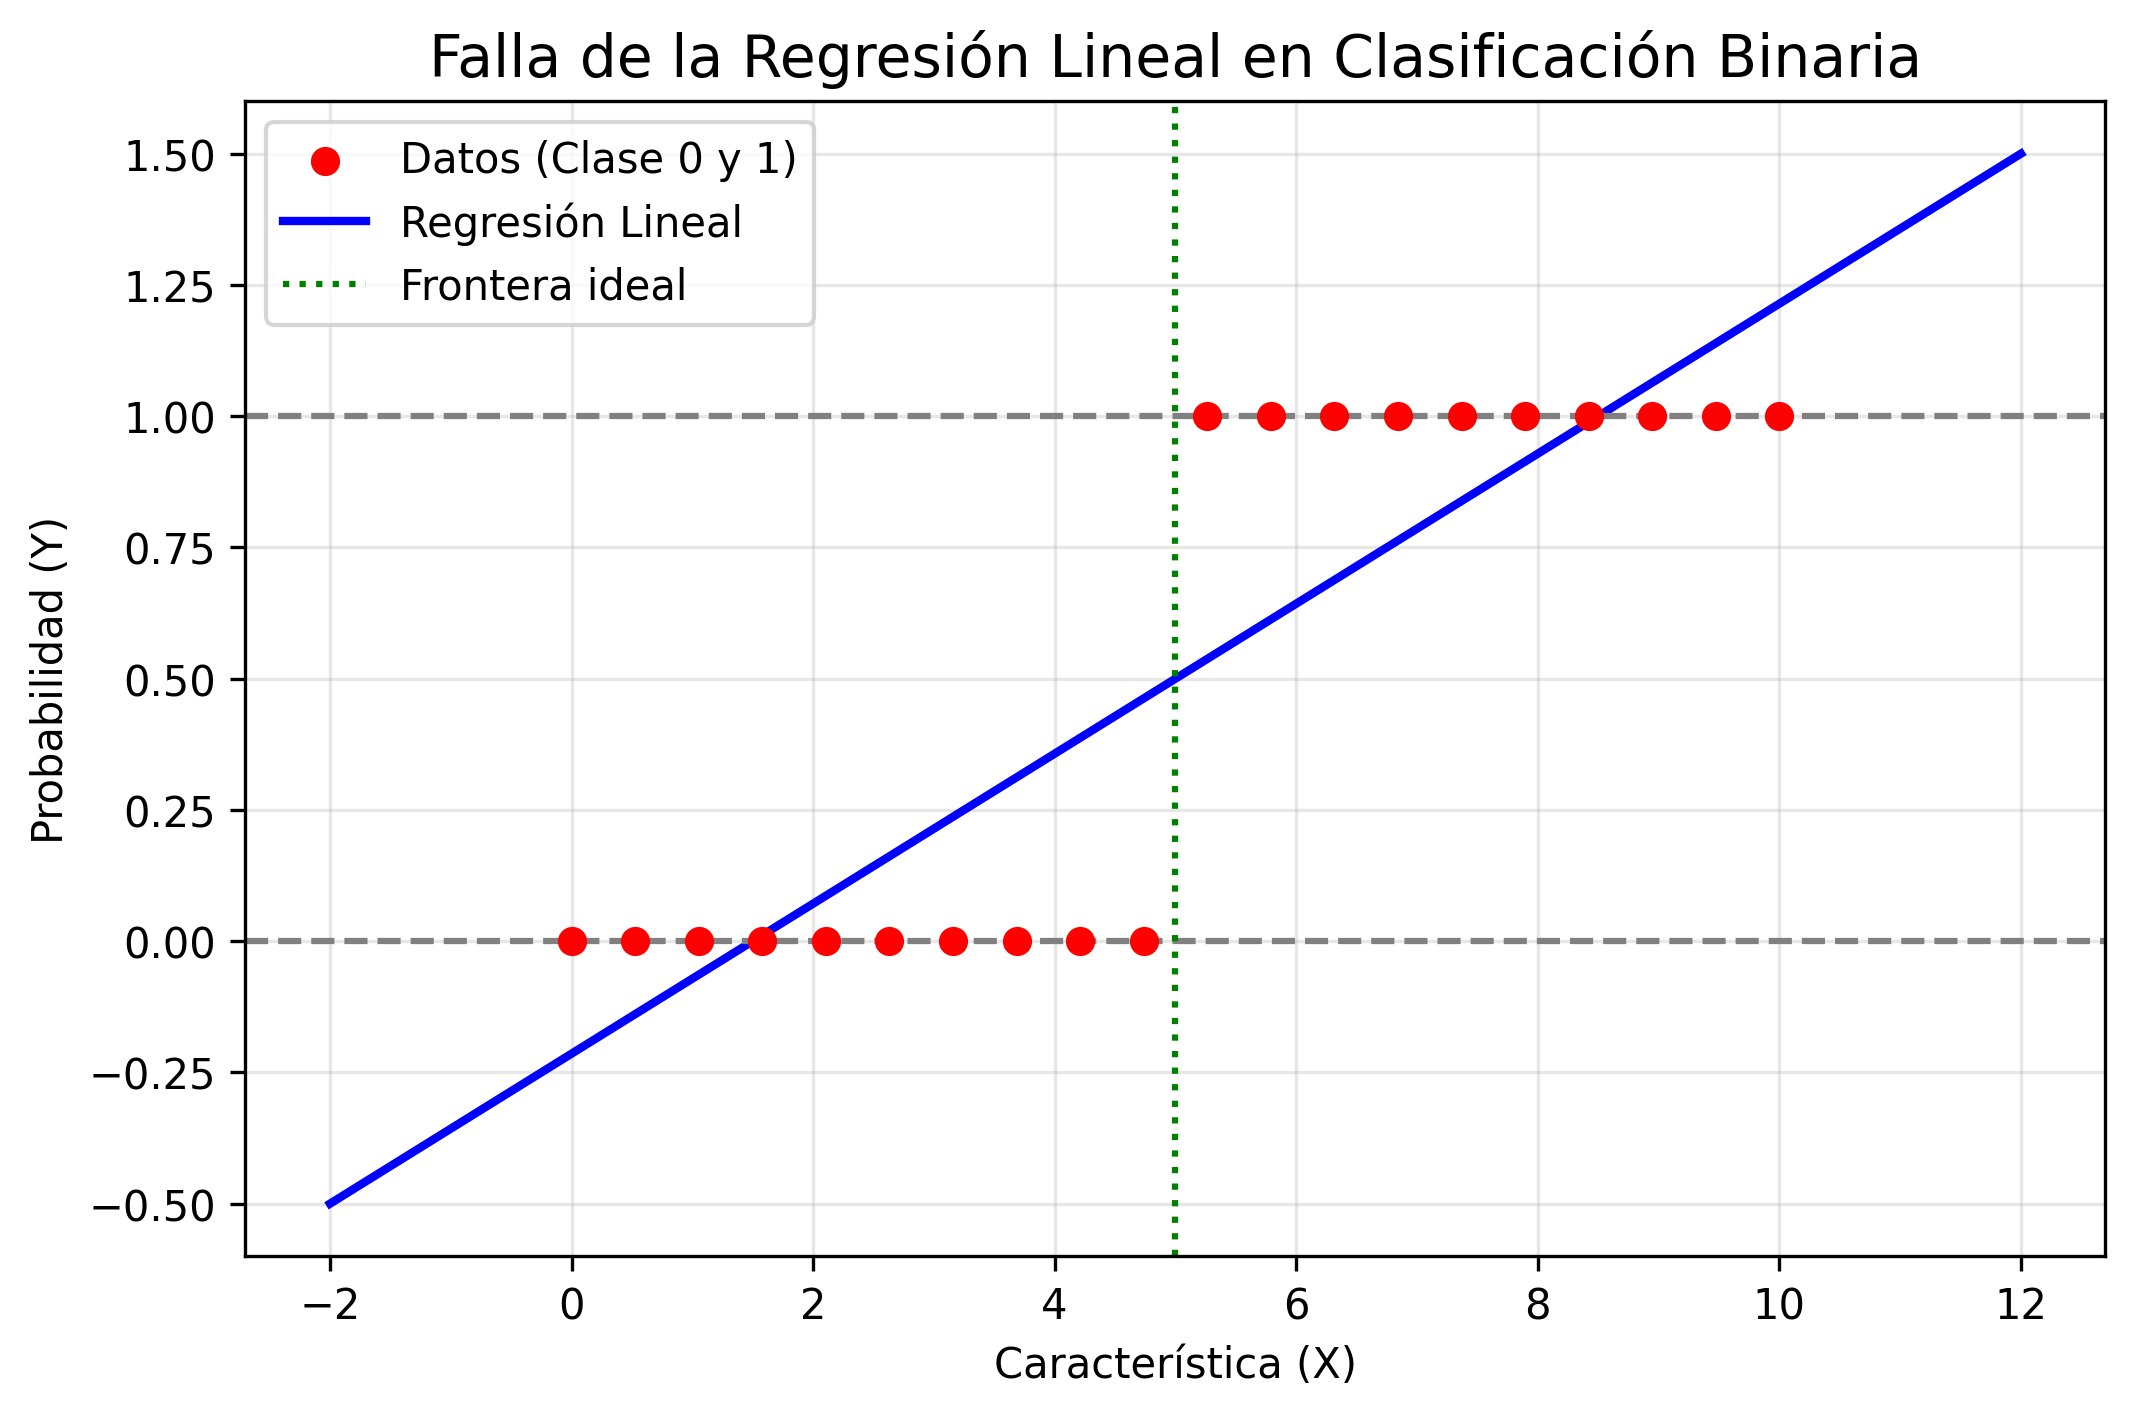
\includegraphics[width=0.85\textwidth,height=0.75\textheight,keepaspectratio]{linear_vs_logistic.png}
    \end{center}
\end{frame}

\begin{frame}{La Función Sigmoide}
    \textbf{Fundamento Matemático:}
    \vspace{0.3cm}
    \\
    Pasamos el resultado de nuestra recta a través de la \textbf{Función Sigmoide}:
    \begin{equation*}
    P(y=1|X) = \frac{1}{1 + e^{-z}}
    \end{equation*}
    Donde $z = \beta_0 + \beta_1 x_1 + ... + \beta_n x_n$.
    
    \begin{itemize}
        \item \textbf{Umbral (Threshold):} Usualmente, si $P \geq 0.5$, predecimos 1. Si $P < 0.5$, predecimos 0.
    \end{itemize}
\end{frame}

\begin{frame}{La Función Sigmoide (Visualización)}
    \begin{center}
        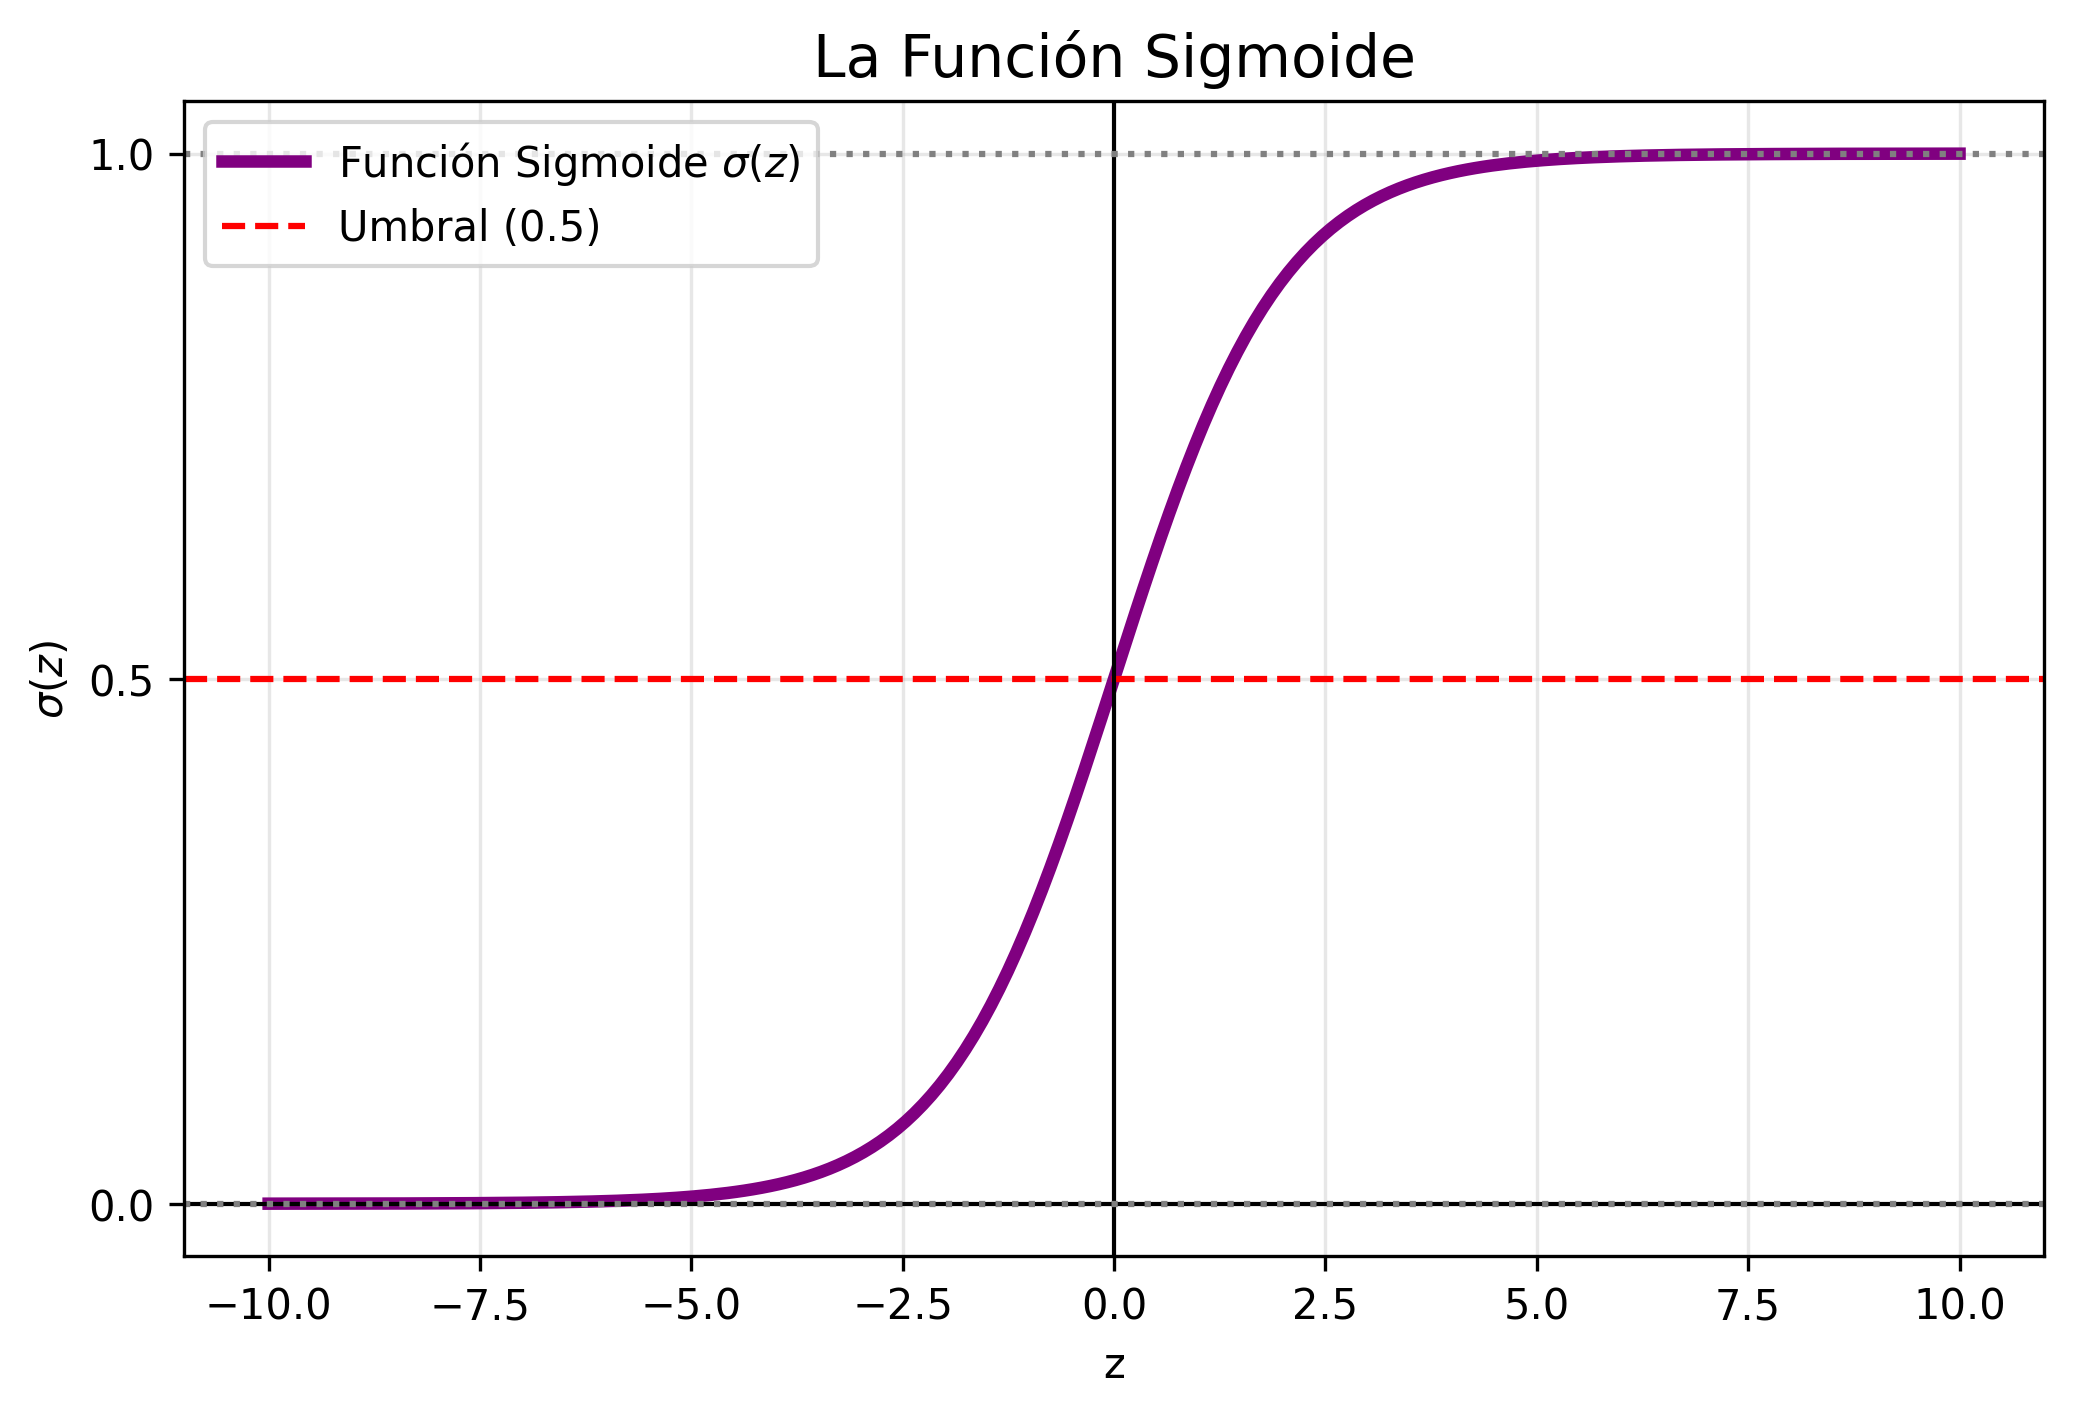
\includegraphics[width=0.85\textwidth,height=0.75\textheight,keepaspectratio]{funcion_sigmoide.png}
    \end{center}
\end{frame}

\begin{frame}{Frontera de Decisión (Decision Boundary)}
    \textbf{Separación en el Espacio Dimensional}
    \vspace{0.3cm}
    \\
    \begin{itemize}
        \item La Regresión Logística crea un \textbf{Hiperplano} (una línea en 2D, un plano en 3D) que corta el espacio.
        \item Este corte ocurre exactamente donde la probabilidad es del 50\% ($P=0.5$).
        \item Separa las instancias clasificadas como positivas de las clasificadas como negativas.
    \end{itemize}
\end{frame}

\begin{frame}{Evaluación: Matriz de Confusión}
    En clasificación, la exactitud (Accuracy) es insuficiente.
    \vspace{0.3cm}
    \begin{table}[]
    \begin{tabular}{|l|l|l|}
    \hline
    \textbf{Real \textbackslash{} Predicción} & \textbf{Predice Negativo (0)} & \textbf{Predice Positivo (1)} \\ \hline
    \textbf{Es Negativo (0)}                  & Verdadero Negativo (VN)      & Falso Positivo (FP)          \\ \hline
    \textbf{Es Positivo (1)}                  & Falso Negativo (FN)          & Verdadero Positivo (VP)      \\ \hline
    \end{tabular}
    \end{table}
    \vspace{0.3cm}
    \begin{itemize}
        \item \textbf{FP (Error Tipo I):} El modelo predice 1, pero era 0.
        \item \textbf{FN (Error Tipo II):} El modelo predice 0, pero era 1.
    \end{itemize}
\end{frame}

\begin{frame}{Métricas de Negocio: Precisión vs Recall}
    Dependiendo del objetivo del negocio, se prioriza una u otra:
    \vspace{0.3cm}
    \begin{itemize}
        \item \textbf{Precisión ($VP / (VP + FP)$):} Calidad. De todos los positivos predichos, ¿cuántos lo son realmente? 
        \begin{itemize}
            \item \textit{Ideal cuando un FP es costoso.}
        \end{itemize}
        \vspace{0.2cm}
        \item \textbf{Sensibilidad o Recall ($VP / (VP + FN)$):} Cantidad. De todos los positivos reales, ¿cuántos logró encontrar el modelo? 
        \begin{itemize}
            \item \textit{Ideal cuando un FN es inaceptable.}
        \end{itemize}
    \end{itemize}
\end{frame}

\begin{frame}[fragile]{Comandos Base: Regresión Logística (Scikit-Learn)}
    \begin{itemize}
        \item \verb|LogisticRegression()|: \textit{Instanciación.} Genera el objeto clasificador configurado para Regresión Logística.
        \item \verb|StandardScaler()|: \textit{Instanciación.} Genera el transformador para estandarizar datos, crucial en regresión logística.
        \item \verb|confusion_matrix(y_test, y_pred)|: \textit{Evaluación.} Calcula la matriz de confusión evaluando las predicciones contra los valores reales.
        \item \verb|classification_report(y_test, y_pred)|: \textit{Evaluación.} Genera un reporte detallado con las métricas de Precisión, Recall y F1-Score para ambas clases.
    \end{itemize}
\end{frame}

\begin{frame}[fragile]
    \begin{center}
        \Large \textbf{Fin de la Presentación Teórica}\\
        \vspace{0.5cm}
        \normalsize Transición al Laboratorio Práctico:\\
        \vspace{0.2cm}
        \verb|04_Regresion_Logistica.ipynb|
    \end{center}
\end{frame}

\end{document}
